\chapter{Topology and Knotting in Soft Matter Systems}

\section{Introduction: Kelvin's vortex atom}
The original, and perhaps most familiar, example of a knotted field is the smoke ring. Easily made by cutting a circular hole in a rectangular box, then replacing the opposite side entirely with a sheet of rubber, ``a blow on this flexible side causes a circular vortex ring to shoot out from the hole on the other side'' \citep{Kelvin}. In 1867, exactly this demonstration was shown to Lord Kelvin by Peter Guthrie Tait. What is generated is a tightly circulating tube of air, closed into a ring, which propagates stably across the room, rebounding elastically from walls and even other vortex rings (of course to see the ring one first needs to fill the box with smoke, perhaps using dry ice or ``a small quantity of muriatic acid'' \citep{Kelvin}). At the time, the microscopic nature of atoms was still under debate, and the stability of the rings, a consquence of Helmholtz's laws of vortex motion in an ideal fluid \citep{Helmholtz} (translated into English by Tait), coupled with their elasticity and capacity for internal vibration \citep{KelvinMasters, KelvinAMS} prompted Kelvin to suggest that ``Helmholtz's rings are the only true atoms". Kelvin hypothesised that such rings, embedded in a ``perfect homogenous liquid''\footnote{Kelvin did not actually specify whether this fluid was the same as the `ether' hypothesised to transmit electromagnetic waves \citep{KelvinMasters}.}, and ``linked together or ...knotted in any manner'' might form the microscopic basis of all matter \citep{Kelvin}.
\begin{figure}[htbp]
\centering
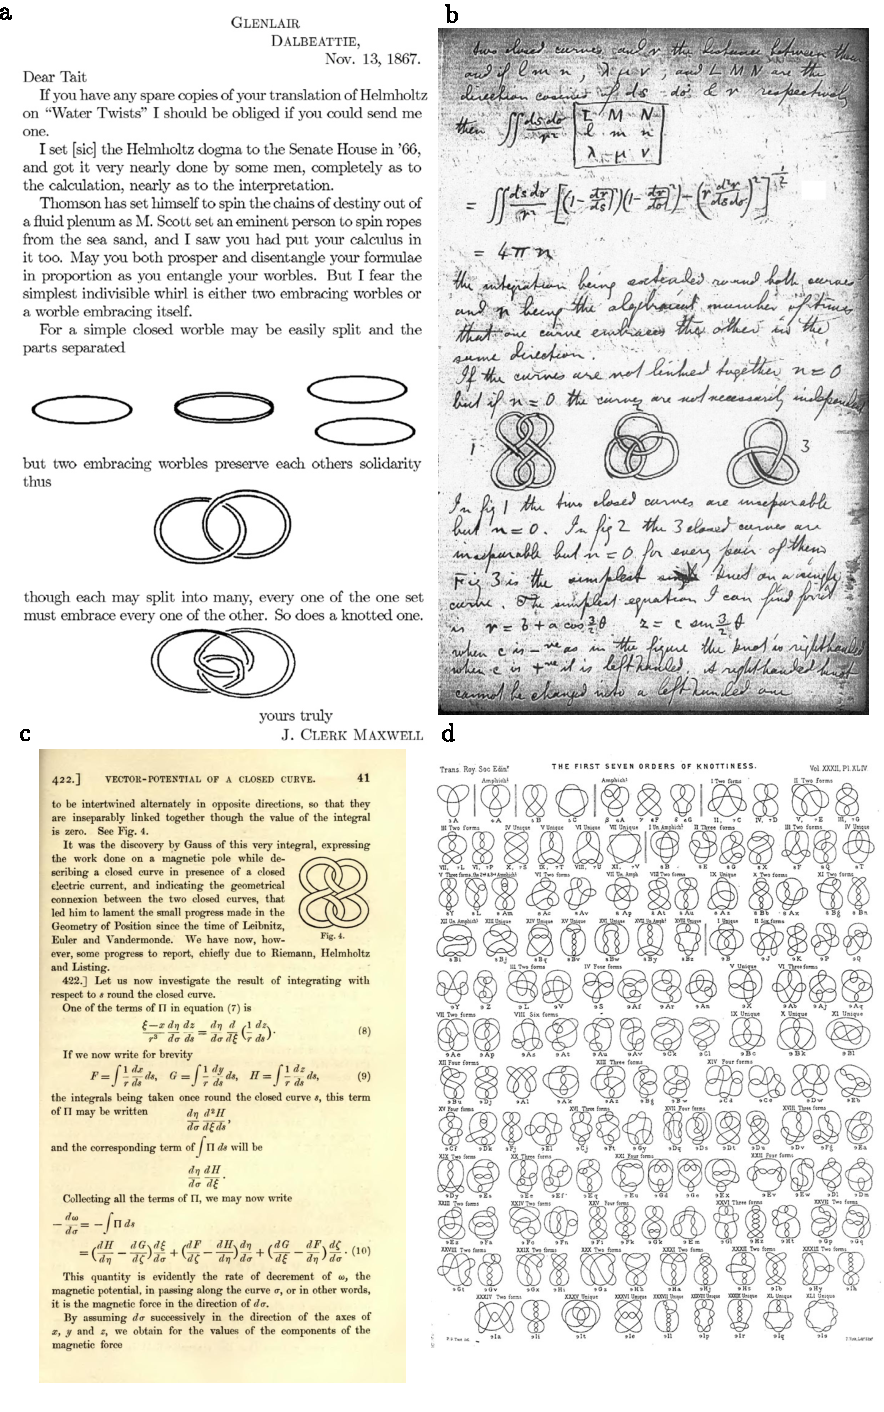
\includegraphics[width=0.99\linewidth]{\IntroductionFigures/History.pdf}
\caption{hi }
\label{fig:History}
\end{figure}

Kelvin's ``vortex atom'' rapidly encountered difficulties in its mathematical content, its falsifiability, and a lack of contempory experimental support \citep{KelvinMasters}. However its content, summarised as ``\textit{Physics = Geometry}'' in Ref. \citep{KelvinAMS}, was compelling (perhaps slightly dangerously so) and apparently motivated Tait, in ``consideration of the forms of knots by Sir W. Thomson's (Lord Kelvin) Theory of Vortex Atoms'', to construct the first systematic tables of knots in 1876--1885 (Figure \ref{fig:History}) \citep{Tait}. Tait's articles, alongside a ``very remarkable essay by Listing ... and an acute remark made by Gauss ... with some comments on it by Clerk-Maxwell'' \citep{Tait}form the initial studies in  what is now the mathematical field of Knot Theory \cite{Lickorish}. Maxwell himself, although not an active contributor to vortex atom theory, had a clear interest in the ideas, encouraging Tait and Kelvin to ``prosper and disentangle your formulae in proportion as you entangle your worbles'' (Figure \ref{fig:History}) \citep{MaxwellTaitLetter}. Indeed the ``comments by Clerk-Maxwell'' referred to by Tait are in fact Maxwell's rederivation of Gauss's Linking number, as presented in his \textit{Treatise on Electricity and Magnetsim} in 1873, about which we will have much more to say in \ref{ch2}. 

Despite forming the starting point for modern knot theory, the knotted structures above are quite different to those found in your shoelaces, or in the world of art and design outside the physics department\footnote{or so I am told.}. Rather than a single knotted curve, we have a continuous fluid in whose structure the knot is encoded, and from which dynamical properties of the knot (its motion, stability, a spectrum of vibrational modes etc.) may be derived. More precisely, we have a concentrated tube of vorticity in the fluid, tied into the shape of a knot. Helmholtz's laws of vortex motion demonstrated that, in a perfect (frictionless) fluid this tube of vorticity was `frozen in' to the fluid, unable to dissapate or cross itself. In an idealised vortex atom, the radius of this tube would tend to zero, with the vorticity contained inside becoming infinite, and we would have a singular linelike structure, tied into a knot and embedded into a continuous three dimensional medium. A structure of this general form is called a \emph{knotted field}, of which the vortex atom may be considered a prototype; as we shall see, such structures are not just confined to fluids. 

The disconnect between a knotted curve and a knotted field is reflected in Tait's work, which mentions Kelvin's Vortex Atoms briefly as motivation, but focuses in substance on ``\emph{the investigation of the essentially different modes of joining points in a plane}'' \citep{Tait}. As knot theory developed, its initial connections to hydrodynamics and electromagnetism were further abandoned. We also note that despite the wonderful knot tables produced by Tait (figure \ref{fig:History}) and the reliance of vortex atom theory on knotted and linked vortices, there is no mention above of any experimental evidence on vortices tied in nontrivial knots. 

\section{Modern knotted fields: experiments}
\begin{figure}[htbp]
\centering
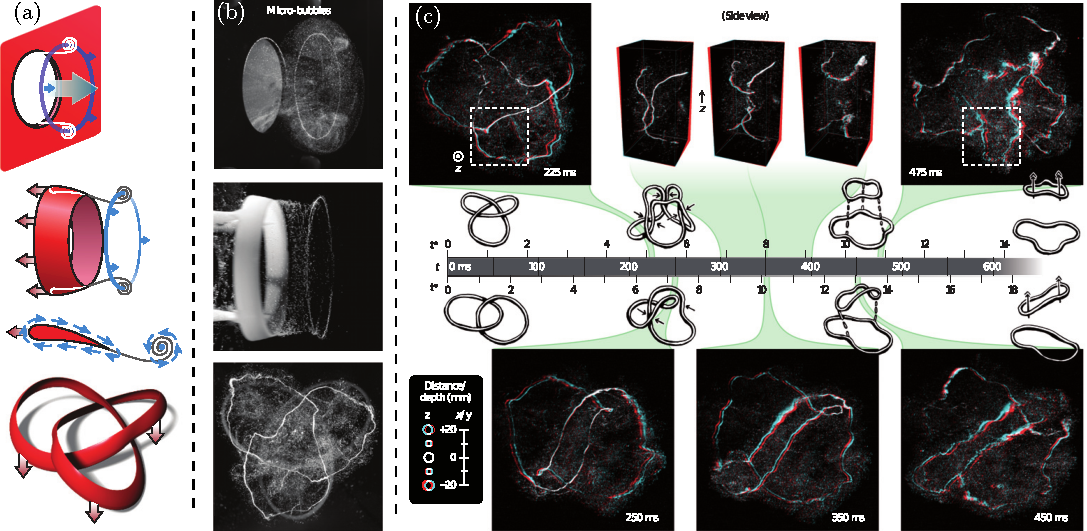
\includegraphics[width=1 \linewidth]{\IntroductionFigures/Irvine_Figs1_3.pdf}
\caption{hi }
\label{fig:Irvine}
\end{figure}
The first experimental construction of nontrivial knotted fluid vortices came 140 years after their initial theoretical investigation, from the Irvine lab in 2013 --- we show in figure \ref{fig:Irvine} several remarkable figures reproduced from Ref.~\citep{Kleckner2013}, in which Kleckner et al. tied a single vortex in water into a trefoil knot, the simplest nontrivial knot, as well as linking two of them together (Kelvin's proposed model for a Sodium atom), before tracking their evolution in full 3D. We postpone a theoretical discussion until \ref{sec:}, but note immeadiately that in a real fluid vortices do not behave like Kelvin's vortex atoms. They are not stable, but rather undergo a series of strand reconnections resulting in multiple disconnected unknots.

Ref.~\citep{Kleckner2013} is a noteable example of a more general trend; over the past $\sim10$ years knotted fields have gone from being purely theoretical constructions to being experimentally realisable in a number of systems, and though originally concieved of in fluid dynamics, modern applications are not limited to this context; they have been realised as nodal lines of optical beams~\cite{Dennis2010} and as disclinations in nematic liquid crystals and spinor Bose-Einstein condensates~\cite{Tkalec2011,Tasinkevych2014,Copar2015}. The liquid crystal system in particular is a primary motivator for this thesis, and in \ref{ch:3} we will discuss knotted fields in a novel form of liquid crystal~\cite{Lavrentovich}, so it is worth giving a detailed description of the experiment; it also provides a second example of a knotted field not arising from hydrodynamics, which we can compare and contrast with the hydrodynamical case.

\subsection{Experiments in liquid crystals}

\begin{figure}[htbp]
\centering
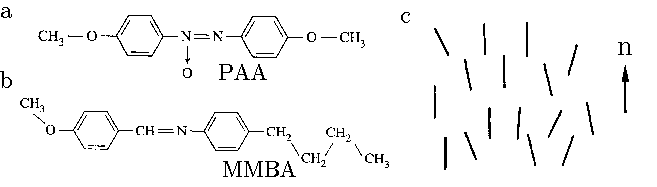
\includegraphics[width=1\linewidth]{\IntroductionFigures/DeGennesMontage.pdf}
\caption{hi }
\label{fig:DeGennesMontage}
\end{figure}

Liquid crystals are a class of materials which possess properties associated to both liquids and solids. In their most common form, the nematic phase, they show no positional order, and flow like a liquid \cite{DeGennes}. However, they do show orientational order: if one attempts to twist a portion of the liquid crystal it will respond elastically, as a solid would (this is remarkable: imagine your surprise if, upon attempting to stir your coffee, you found it fiercly resisted your attempts to turn the spoon, but was nevertheless happy to be poured down the sink). The molecules which comprise nematics, two examples of which are shown in Figure \ref{fig:DeGennesMontage}, are typically thin rods which align themselves along some common axis. In continuum theories this orientational order is described by a spatially varying unit vector field $\bf n$, called the director, which represents an average local molecular orientation, as shown in Figure \ref{fig:DeGennesMontage} (c). For our purposes, the most interesting thing about this order is where it breaks down; a celebrated feature of liquid crystals are their topological defects, places in the material where the director is undefined. These defects may be easily seen in a 2D slice of nematic placed between cross polarisers, creating a Schlieren texture \cite{DeGennes} like the one shown in figure \ref{fig:Disclination}(e). Places in the sample where the director is aligned with one of the two shown polarizer directions H and V will not transmit light, leading to the dark brushed observed. At points where these brushes meet, we cannot define the director; these are the defects. Note immeadiately that some defects have four brushes entering them, some only have two. Traversing a circle around a defect with two brushes, the director is aligned with each of H and V only once; in other word it makes only half a turn in a full circle around the defect. This observation is enough to establish that the dierctor $\bf{n}$ must in fact be non-orientable; it should not be thought of as a vector field, but as a line field, for which $\bf n \sim - \bf n$. In figure \ref{fig:Disclination} (a)--(d) we show configurations of the director around these defects, with their associated Schlieren texture brushes. In (a) and (d) we have four brushes, and a line field which can be oriented; to emphasise this fact we have decorated the line field with one of the two possible choices of arrowheads. Figures (b) and (c) correspond to the non-orientable two brush case; here one cannot consistently assign arrowheads to the rods (it is worth trying to imagine doing so). In two dimensions these defects are points, in three dimensions they are lines called disclinations, transverse cross sections of which have local profiles resembling the two dimensional case; a schematic illustration of such a disclination is shown in Figure \ref{fig:Disclination}(f). 
\begin{figure}[htbp]
\centering
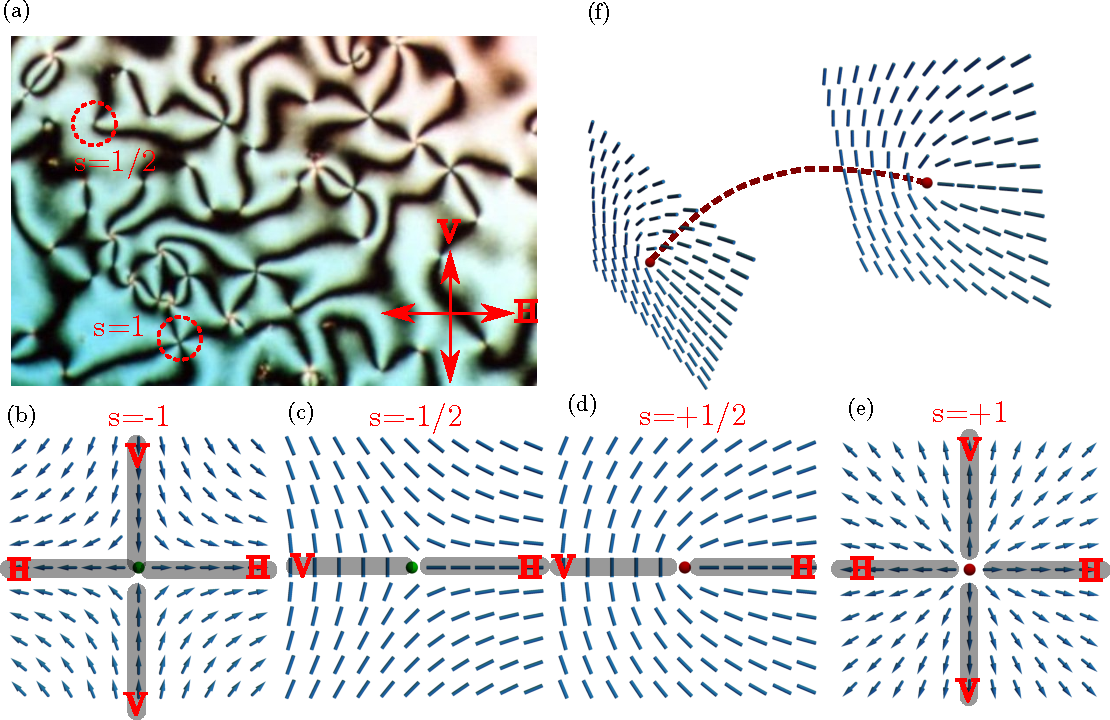
\includegraphics[width=1\linewidth]{\IntroductionFigures/DisclinationLine.pdf}
\caption{hi }
\label{fig:Disclination}
\end{figure}

One of the major advantages of working with liquid crystal disclinations is the fine control experimentalists have over them. The disclinations shrink under line tension \cite{Tkalec2011} effectively acting as microscopic rubber bands, and may be manipulated using lazer tweezers. In order to stabilise against contraction, Refs.~\cite{Tkalec2011,Tasinkevych2014,Copar2015} wrap them around colloidal inclusions of diameter $4.72$ $\mu$m within a 5.5 $\mu$m thick slab of liquid crystal; Figure \ref{fig:KnottedLiquidCrystal} shows an example of the lazer tweezer manipulation of these `Saturn's rings'. Remarkably, when two of these colloids are brought together, the disclinations, either spontaneously or induced by the tweezers, fuse together. Assembling an array of these colloids as in \ref{fig:KnottedLiquidCrystal)} (b) and weaving the disclination lines around them, this setup allows targeted construction of certain knotted and linked tangles; examples of some possible link topologies are shown in Figure \ref{fig:KnottedLiquidCrystal} (b). This system also illustrates that knotted fields are more complex than a single knotted curve; this curve organises the entire field  (in this case the director $\bf n$) around it. Figure \ref{fig:KnottedLiquidCrystal}(c) shows one such colloidal tangle under a $\lambda$ plate, which allows one to distinguish regions where the director $\bf n$ is twisting in either a right or left handed sense by the colouring of the image. We see that the disclinations separate regions of the liquid crystal into alternately right and left handed regions. This division allows construction of a surface spanning the disclinations, called the Pontryagin-Thom surface \cite{Chen}, which allows complete classification of the topology of this liquid crystal texture; for any fixed knotted disclination, there may in fact be several director configurations which cannot be deformed continuously into one another \cite{Machon}, and the Pontryagin-Thom surface detects this. 

%In the system of Refs.~\cite{Tkalec2011,Tasinkevych2014,Copar2015} these disclinations are the line-like structures analogous to fluid vortex filaments, with the director $\bf n$ supporting them in anology, topologically speaking, to the fluid velocity.
\begin{figure}[htbp]
\centering
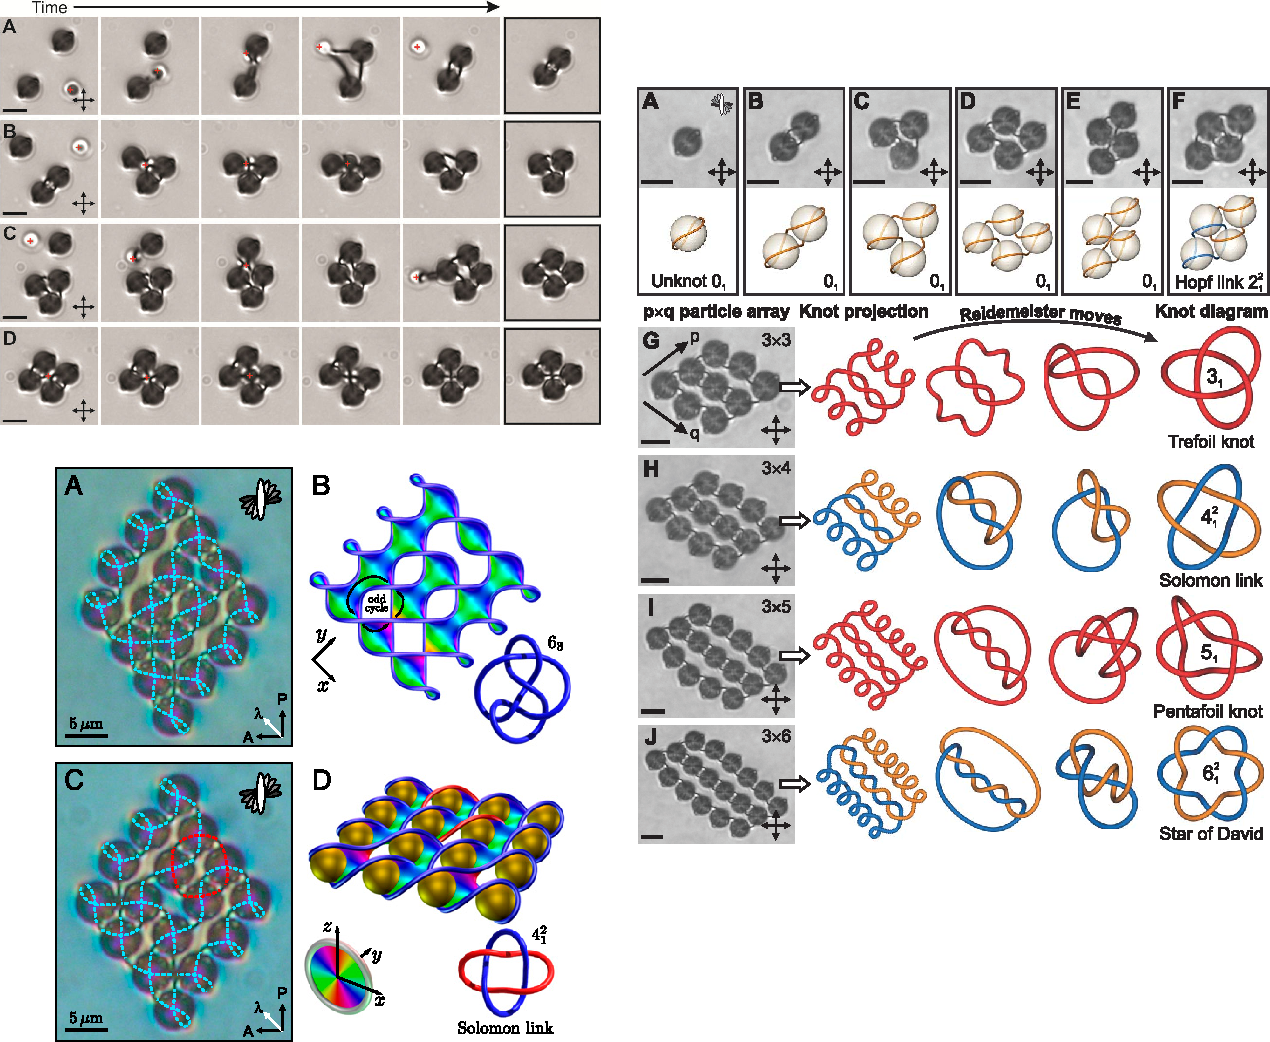
\includegraphics[width=1 \linewidth]{\IntroductionFigures/LiquidCrystalMontage.pdf}
\caption{hi }
\label{fig:KnottedLiquidCrystal}
\end{figure}

\section{Modern knotted fields: theory and simulation}

%We immeadiately note that in contrast to Helmholtz and Kelvin's ideal fluid, in a real fluid knots do not persist indefinitely but untie over time. 

